\section{Ergebnisse}
\label{ergebnisse}

% 10.000 Steps mit Batch Size 64\\
% Learning-Rate: 0.001\\
% Dropout: 0.5\\

% \begin{tabular}{cccc}
%   \toprule
%   Verfahren & Netzarchitektur & Dauer & Genauigkeit\\
%   \midrule
%   klassisch & C5-32-P4-C5-64-P4-FC1024 & 0.18s & 99.189\\
%   klassisch & C32-C32-P4-C64-C64-P4-FC1024 & 0.25s & 99.139\\
%   Chebyshev & C25-32-P4-C25-64-P4-FC1024 & 0.91s & 98.888\\
%   GCN & C32-C32-P4-C64-C64-P4-FC1024 & 0.22s & 96.675\\
%   E-GCN & C32-C32-P4-C64-C64-P4-FC1024 & 0.77s & 99.145\\
%   \bottomrule
% \end{tabular}
% \todo{fuckin patchy}

% \paragraph{Vergleich \bzgl{} vorhandener Implementierungen}
% \label{vergleich_ergebnisse}

% PascalVOC Squeeze einheitliche Größe von $224 \times 224$.

% \paragraph{\gls{Cifar}-10}

% Abbildung~\ref{fig:cifar_10_train} zeigt
\begin{figure}[t]
\centering
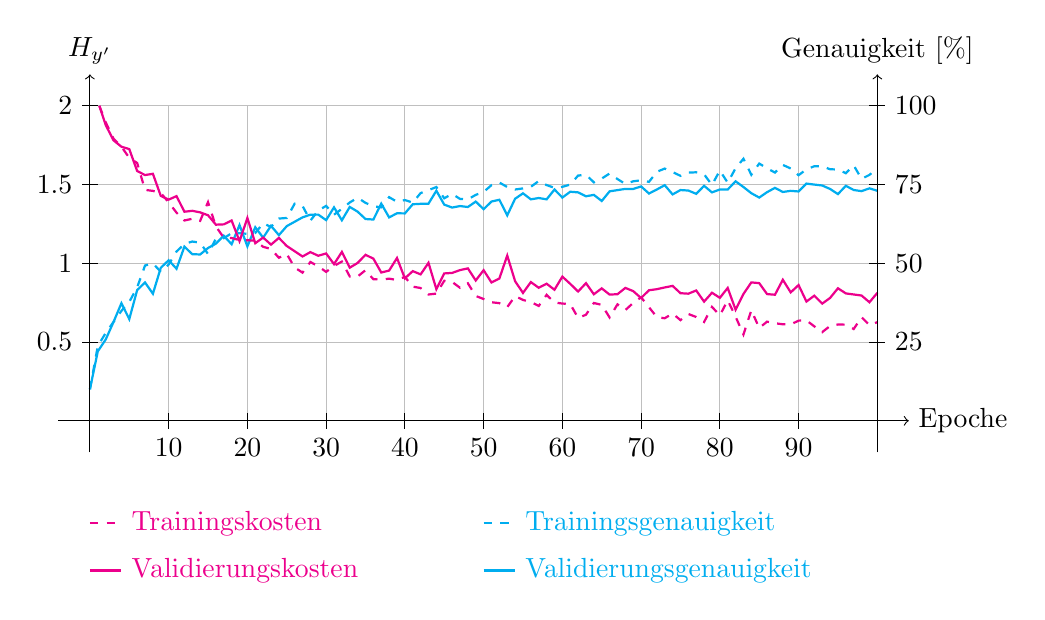
\begin{tikzpicture}
  \draw[color=lightgray] (0, 0) grid (10, 4);

  \tikzstyle{color1}=[color=cyan]
  \tikzstyle{color2}=[color=magenta]

  % Train accuracy.
  \draw[color1, dashed, thick] (0, 0.4) -- (0.1, 0.95) -- (0.2, 1.1146) -- (0.3, 1.2557) -- (0.4, 1.3958) -- (0.5, 1.5104) -- (0.6, 1.6944) -- (0.7, 1.9722) -- (0.8, 2.0) -- (0.9, 1.892) -- (1.0, 1.9844) -- (1.1, 2.15) -- (1.2, 2.2452) -- (1.3, 2.2768) -- (1.4, 2.2625) -- (1.5, 2.1181) -- (1.6, 2.3125) -- (1.7, 2.3188) -- (1.8, 2.3828) -- (1.9, 2.3819) -- (2.0, 2.375) -- (2.1, 2.3854) -- (2.2, 2.5089) -- (2.3, 2.4615) -- (2.4, 2.5682) -- (2.5, 2.5764) -- (2.6, 2.7569) -- (2.7, 2.7292) -- (2.8, 2.5417) -- (2.9, 2.6711) -- (3.0, 2.7292) -- (3.1, 2.6172) -- (3.2, 2.6927) -- (3.3, 2.7727) -- (3.4, 2.8333) -- (3.5, 2.7679) -- (3.6, 2.725) -- (3.7, 2.7109) -- (3.8, 2.8403) -- (3.9, 2.7812) -- (4.0, 2.8036) -- (4.1, 2.7708) -- (4.2, 2.892) -- (4.3, 2.9297) -- (4.4, 2.9688) -- (4.5, 2.8259) -- (4.6, 2.8819) -- (4.7, 2.8182) -- (4.8, 2.8125) -- (4.9, 2.8693) -- (5.0, 2.9062) -- (5.1, 2.9931) -- (5.2, 3.026) -- (5.3, 2.9688) -- (5.4, 2.9375) -- (5.5, 2.9514) -- (5.6, 2.9716) -- (5.7, 3.0455) -- (5.8, 2.9937) -- (5.9, 2.9583) -- (6.0, 2.9716) -- (6.1, 3.0) -- (6.2, 3.1146) -- (6.3, 3.125) -- (6.4, 3.0284) -- (6.5, 3.0764) -- (6.6, 3.1406) -- (6.7, 3.0703) -- (6.8, 3.0078) -- (6.9, 3.0417) -- (7.0, 3.0547) -- (7.1, 3.0341) -- (7.2, 3.1625) -- (7.3, 3.2031) -- (7.4, 3.1597) -- (7.5, 3.1111) -- (7.6, 3.1518) -- (7.7, 3.1562) -- (7.8, 3.1302) -- (7.9, 2.9948) -- (8.0, 3.1786) -- (8.1, 3.0234) -- (8.2, 3.2083) -- (8.3, 3.3281) -- (8.4, 3.125) -- (8.5, 3.267) -- (8.6, 3.2067) -- (8.7, 3.1528) -- (8.8, 3.25) -- (8.9, 3.2045) -- (9.0, 3.1187) -- (9.1, 3.1938) -- (9.2, 3.233) -- (9.3, 3.233) -- (9.4, 3.1944) -- (9.5, 3.1917) -- (9.6, 3.1445) -- (9.7, 3.2437) -- (9.8, 3.0729) -- (9.9, 3.123) -- (10, 3.208);

  % Validation accuracy.
  \draw[color1, thick] (0, 0.4) -- (0.1, 0.8812) -- (0.2, 1.0312) -- (0.3, 1.2557) -- (0.4, 1.4931) -- (0.5, 1.2917) -- (0.6, 1.6597) -- (0.7, 1.7569) -- (0.8, 1.6136) -- (0.9, 1.9432) -- (1.0, 2.0391) -- (1.1, 1.9312) -- (1.2, 2.2115) -- (1.3, 2.1161) -- (1.4, 2.1125) -- (1.5, 2.1944) -- (1.6, 2.25) -- (1.7, 2.35) -- (1.8, 2.2422) -- (1.9, 2.4861) -- (2.0, 2.2153) -- (2.1, 2.4583) -- (2.2, 2.3259) -- (2.3, 2.476) -- (2.4, 2.358) -- (2.5, 2.4722) -- (2.6, 2.5278) -- (2.7, 2.5833) -- (2.8, 2.6181) -- (2.9, 2.6184) -- (3.0, 2.5486) -- (3.1, 2.7109) -- (3.2, 2.5469) -- (3.3, 2.7159) -- (3.4, 2.6562) -- (3.5, 2.5625) -- (3.6, 2.5562) -- (3.7, 2.7578) -- (3.8, 2.5833) -- (3.9, 2.6354) -- (4.0, 2.6339) -- (4.1, 2.75) -- (4.2, 2.7557) -- (4.3, 2.7578) -- (4.4, 2.9219) -- (4.5, 2.7455) -- (4.6, 2.7083) -- (4.7, 2.7273) -- (4.8, 2.7153) -- (4.9, 2.7841) -- (5.0, 2.6875) -- (5.1, 2.7847) -- (5.2, 2.8073) -- (5.3, 2.6094) -- (5.4, 2.8203) -- (5.5, 2.8889) -- (5.6, 2.8125) -- (5.7, 2.8295) -- (5.8, 2.8125) -- (5.9, 2.9375) -- (6.0, 2.8352) -- (6.1, 2.9091) -- (6.2, 2.901) -- (6.3, 2.8516) -- (6.4, 2.8693) -- (6.5, 2.7917) -- (6.6, 2.9141) -- (6.7, 2.9297) -- (6.8, 2.9453) -- (6.9, 2.9444) -- (7.0, 2.9766) -- (7.1, 2.8864) -- (7.2, 2.9375) -- (7.3, 2.9922) -- (7.4, 2.875) -- (7.5, 2.9306) -- (7.6, 2.9241) -- (7.7, 2.8828) -- (7.8, 2.9844) -- (7.9, 2.901) -- (8.0, 2.9375) -- (8.1, 2.9375) -- (8.2, 3.0417) -- (8.3, 2.9688) -- (8.4, 2.8906) -- (8.5, 2.8352) -- (8.6, 2.9038) -- (8.7, 2.9583) -- (8.8, 2.9062) -- (8.9, 2.9205) -- (9.0, 2.9125) -- (9.1, 3.0125) -- (9.2, 3.0) -- (9.3, 2.9886) -- (9.4, 2.9444) -- (9.5, 2.8792) -- (9.6, 2.9844) -- (9.7, 2.9312) -- (9.8, 2.9167) -- (9.9, 2.9523) -- (10, 2.9214);

  % Train loss.
  \draw[color2, dashed, thick] (0.12, 4) -- (0.2, 3.7924) -- (0.3, 3.5816) -- (0.4, 3.4817) -- (0.5, 3.339) -- (0.6, 3.2744) -- (0.7, 2.933) -- (0.8, 2.92) -- (0.9, 2.893) -- (1.0, 2.7748) -- (1.1, 2.6434) -- (1.2, 2.5438) -- (1.3, 2.566) -- (1.4, 2.5388) -- (1.5, 2.7772) -- (1.6, 2.4688) -- (1.7, 2.3255) -- (1.8, 2.3209) -- (1.9, 2.2951) -- (2.0, 2.2934) -- (2.1, 2.2871) -- (2.2, 2.2098) -- (2.3, 2.182) -- (2.4, 2.0707) -- (2.5, 2.1185) -- (2.6, 1.9472) -- (2.7, 1.882) -- (2.8, 2.017) -- (2.9, 1.962) -- (3.0, 1.8913) -- (3.1, 1.9663) -- (3.2, 2.0222) -- (3.3, 1.8329) -- (3.4, 1.833) -- (3.5, 1.9122) -- (3.6, 1.7979) -- (3.7, 1.7941) -- (3.8, 1.8049) -- (3.9, 1.7891) -- (4.0, 1.8278) -- (4.1, 1.7039) -- (4.2, 1.6864) -- (4.3, 1.6041) -- (4.4, 1.6157) -- (4.5, 1.7782) -- (4.6, 1.7638) -- (4.7, 1.6894) -- (4.8, 1.7469) -- (4.9, 1.5853) -- (5.0, 1.547) -- (5.1, 1.5054) -- (5.2, 1.4945) -- (5.3, 1.4434) -- (5.4, 1.5836) -- (5.5, 1.5352) -- (5.6, 1.5082) -- (5.7, 1.4586) -- (5.8, 1.5991) -- (5.9, 1.5021) -- (6.0, 1.4892) -- (6.1, 1.483) -- (6.2, 1.307) -- (6.3, 1.3468) -- (6.4, 1.4963) -- (6.5, 1.4723) -- (6.6, 1.3129) -- (6.7, 1.4788) -- (6.8, 1.4064) -- (6.9, 1.4973) -- (7.0, 1.5687) -- (7.1, 1.4423) -- (7.2, 1.317) -- (7.3, 1.3022) -- (7.4, 1.3634) -- (7.5, 1.2786) -- (7.6, 1.3565) -- (7.7, 1.3183) -- (7.8, 1.2549) -- (7.9, 1.447) -- (8.0, 1.3388) -- (8.1, 1.5304) -- (8.2, 1.3225) -- (8.3, 1.0959) -- (8.4, 1.4044) -- (8.5, 1.1791) -- (8.6, 1.2593) -- (8.7, 1.2394) -- (8.8, 1.2256) -- (8.9, 1.2238) -- (9.0, 1.2721) -- (9.1, 1.2754) -- (9.2, 1.1993) -- (9.3, 1.1261) -- (9.4, 1.2046) -- (9.5, 1.2231) -- (9.6, 1.2211) -- (9.7, 1.1656) -- (9.8, 1.3159) -- (9.9, 1.2148) -- (10, 1.2526);

  % Validation loss.
  \draw[color2, thick] (0.12, 4) -- (0.2, 3.7574) -- (0.3, 3.5618) -- (0.4, 3.4812) -- (0.5, 3.4506) -- (0.6, 3.1727) -- (0.7, 3.121) -- (0.8, 3.137) -- (0.9, 2.8564) -- (1.0, 2.8091) -- (1.1, 2.8534) -- (1.2, 2.6553) -- (1.3, 2.6668) -- (1.4, 2.6473) -- (1.5, 2.6105) -- (1.6, 2.4908) -- (1.7, 2.4949) -- (1.8, 2.5435) -- (1.9, 2.2812) -- (2.0, 2.5756) -- (2.1, 2.2554) -- (2.2, 2.3275) -- (2.3, 2.2373) -- (2.4, 2.3227) -- (2.5, 2.22) -- (2.6, 2.1535) -- (2.7, 2.087) -- (2.8, 2.1421) -- (2.9, 2.0962) -- (3.0, 2.1254) -- (3.1, 1.9896) -- (3.2, 2.1447) -- (3.3, 1.9447) -- (3.4, 2.0049) -- (3.5, 2.108) -- (3.6, 2.0597) -- (3.7, 1.8835) -- (3.8, 1.908) -- (3.9, 2.0677) -- (4.0, 1.8087) -- (4.1, 1.9008) -- (4.2, 1.8596) -- (4.3, 2.0063) -- (4.4, 1.6715) -- (4.5, 1.8716) -- (4.6, 1.8781) -- (4.7, 1.9138) -- (4.8, 1.9358) -- (4.9, 1.7821) -- (5.0, 1.9127) -- (5.1, 1.7567) -- (5.2, 1.8072) -- (5.3, 2.0986) -- (5.4, 1.7727) -- (5.5, 1.624) -- (5.6, 1.7619) -- (5.7, 1.6896) -- (5.8, 1.7412) -- (5.9, 1.6644) -- (6.0, 1.8309) -- (6.1, 1.7395) -- (6.2, 1.6417) -- (6.3, 1.748) -- (6.4, 1.607) -- (6.5, 1.6818) -- (6.6, 1.6032) -- (6.7, 1.6078) -- (6.8, 1.688) -- (6.9, 1.6468) -- (7.0, 1.5591) -- (7.1, 1.6582) -- (7.2, 1.6715) -- (7.3, 1.6938) -- (7.4, 1.7135) -- (7.5, 1.6207) -- (7.6, 1.6145) -- (7.7, 1.6552) -- (7.8, 1.5135) -- (7.9, 1.6266) -- (8.0, 1.562) -- (8.1, 1.6873) -- (8.2, 1.4112) -- (8.3, 1.611) -- (8.4, 1.7578) -- (8.5, 1.7484) -- (8.6, 1.6091) -- (8.7, 1.6011) -- (8.8, 1.7912) -- (8.9, 1.6309) -- (9.0, 1.724) -- (9.1, 1.5145) -- (9.2, 1.589) -- (9.3, 1.4882) -- (9.4, 1.5603) -- (9.5, 1.6832) -- (9.6, 1.6179) -- (9.7, 1.6045) -- (9.8, 1.591) -- (9.9, 1.5056) -- (10, 1.6248);

  \draw (0.1, 4) -- (-0.1, 4) node[left] {$2$};
  \draw (0.1, 3) -- (-0.1, 3) node[left] {$1.5$};
  \draw (0.1, 2) -- (-0.1, 2) node[left] {$1$};
  \draw (0.1, 1) -- (-0.1, 1) node[left] {$0.5$};

  \draw (9.9, 4) -- (10.1, 4) node[right] {$100$};
  \draw (9.9, 3) -- (10.1, 3) node[right] {$75$};
  \draw (9.9, 2) -- (10.1, 2) node[right] {$50$};
  \draw (9.9, 1) -- (10.1, 1) node[right] {$25$};

  \draw (1, 0.1) -- (1, -0.1)  node[below] {$10$};
  \draw (2, 0.1) -- (2, -0.1)  node[below] {$20$};
  \draw (3, 0.1) -- (3, -0.1)  node[below] {$30$};
  \draw (4, 0.1) -- (4, -0.1)  node[below] {$40$};
  \draw (5, 0.1) -- (5, -0.1)  node[below] {$50$};
  \draw (6, 0.1) -- (6, -0.1)  node[below] {$60$};
  \draw (7, 0.1) -- (7, -0.1)  node[below] {$70$};
  \draw (8, 0.1) -- (8, -0.1)  node[below] {$80$};
  \draw (9, 0.1) -- (9, -0.1)  node[below] {$90$};

  \draw[->] (-0.4, 0)    -- (10.4, 0)   node[right] {Epoche};
  \draw[->] (0,    -0.4) -- (0,    4.4) node[above] {$H_{y^{\prime}}$};
  \draw[->] (10,   -0.4) -- (10,   4.4) node[above] {Genauigkeit [\%]};

  \draw[color2, thick, dashed] (0, -1.3) -- (0.4, -1.3) node[right] {Trainingskosten};
  \draw[color2, thick]         (0, -1.9) -- (0.4, -1.9) node[right] {Validierungskosten};
  \draw[color1, thick, dashed] (5, -1.3) -- (5.4, -1.3) node[right] {Trainingsgenauigkeit};
  \draw[color1, thick]         (5, -1.9) -- (5.4, -1.9) node[right] {Validierungsgenauigkeit};

\end{tikzpicture}
\caption[\gls{Cifar}-10 Kosten- und Genauigkeitsverlauf]{Kosten- und Genauigkeitsverlauf eines Trainings auf dem \gls{Cifar}-10 Datensatz mit dem spektralen Faltungsoperator auf Graphen im zweidimensionalen euklidischen Raum, welche über Quickshift generiert wurden.
Die gestrichelten Linien zeigen die Kosten und Genauigkeiten des Trainingsdatensatzes in Abhängigkeit der Epochen, wohingegen die durchgezogenen Linien sich auf den Validierungsdatensatz beziehen.
Nach der $60$ten Epoche stellt sich eine deutliche Verlangsamung der Lerngeschwindigkeit ein.}
\label{fig:cifar_10_train}
\end{figure}


% Postprocessing weitaus besser als preprocessing!

% Mit drei mal Dropout kein Overfitting, trainiert allerdings langsam
% Learning Rate Decay darf nicht zu krass sein

% Durchschnittliche Faltungsdauer: 2.05s, Preprocessingdauer: 0.35s
% Bei Batch-Size 64
% Erstes Resultat mit Postprocessing:
% Loss: 1.05440, acc: 0.63411

% Zweiter Test:
% Dropout nur noch 2 mal, nicht so starkes Learning Rate Decay
% ist nun bei 70 \% nach 50k Steps
% Dropout ist immer noch zu hart

% 0.82699 loss, acc: .72917

% Alle Faltungen wurden dabei mit einer Partitionsgröße von $8$ bei $K=0$ und $K=1$ implementiert, um ein \gls{CNN} mit einem $3 \times 3$ Filter zu simulieren.
% Es erscheint jedoch vorstellbar die Filtergröße bei größerer lokaler Kontrollierbarkeit, \dhe{} $K > 1$, weiter zu reduzieren und die Gefahr des Overfittings damit aufgrund der kleineren Anzahl an Trainingsparametern einzuschränken.
